%%%%%%%%%%%%%%%%%%%%%%%%%%%%%%%%%%%%%%%%%%%%%%%%%%%%%%%%%%%%%%%%
%% Author: Anshuman Dhuliya (144050002)
%% Document: CV
%% Title: Anshuman Dhuliya CV
%% Commands:
%%     make             # produces the main.pdf file
%%     make clean       # cleans the temporary files
%%     make tar         # makes the tgz file containing all necessary contents
%%     make show        # shows the pdf on evince
%% use: `convert a.jpg eps2:a.eps`  %% to insert jpeg images as eps
%% use: `identify a.eps` command to find the dimensions of a.eps
%%%%%%%%%%%%%%%%%%%%%%%%%%%%%%%%%%%%%%%%%%%%%%%%%%%%%%%%%%%%%%%%
% openright works only with twoside, it opens each chapter on the right side
\documentclass[a4paper,12pt]{article}
%\usepackage{report} %% report.sty HAS ALL THE CONFIGURATIONS
\newcommand{\Space}{\hspace{1ex}}
\newcommand{\Sp}{\hspace{1ex}}
\newcommand{\Heading}[1]{\textbf{\itshape\normalsize #1}}


\usepackage[a4paper,lmargin=1.2cm,rmargin=1.2cm,tmargin=1.5cm,bmargin=1.5cm]{geometry}
\usepackage{tabu}

\usepackage{array}
\newcolumntype{M}[1]{>{\centering\arraybackslash}m{#1}}
\newcolumntype{R}[1]{>{\raggedleft\arraybackslash}m{#1}}

\usepackage{fancyhdr}
\pagestyle{fancy}
\rfoot{\textit{If you can read this, thank a Teacher! -- Anonymous}\Sp{}\Sp{}\Sp{}\Sp{}\Sp{}\Sp{}\textbf{\LaTeX}}
\renewcommand{\headrulewidth}{0pt}

\setlength\tabcolsep{0pt}

\usepackage{graphicx}

\begin{document}
\begin{flushleft}

\pagenumbering{gobble} % no page numbers


%    \begin{tabular}{|l{0.75\textwidth}|l{0.25\textwidth}|}
    \begin{tabular*}{\textwidth}{m{0.85\textwidth} m{0.15\textwidth} }
        {\LARGE{}\rule[3ex]{0ex}{0ex}\textbf{Anshuman Dhuliya}}\newline%
        {\rule[3ex]{0ex}{0ex}\large{}\itshape{}Research Scholar, IIT Bombay, CSE Department} \newline%
        \rule[3ex]{0ex}{0ex}{320 Ground Floor, Type-1 Bldg, Behind H6\newline%
IIT Bombay Campus, Mumbai, Maharashtra, 400076\newline%
        Mob: +91 90045 21241, anshumandhuliya@gmail.com, dhuliya@cse.iitb.ac.in}

&  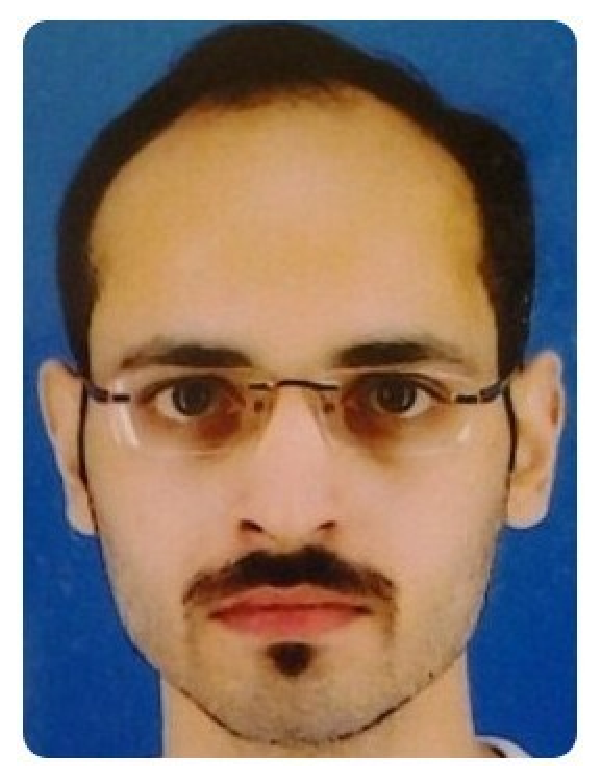
\includegraphics[natwidth=273,natheight=360,width=0.15\textwidth]{images/anshuman1.eps} \\
\end{tabular*}
\rule[1pt]{\textwidth}{2pt}
\begin{tabular*}{\textwidth}{m{0.95\textwidth} m{0.05\textwidth} }
{\itshape{}\rule[3ex]{0ex}{0ex}My objective is to become an expert in my field of interest and foster understanding, passion and\newline%
    self-learning ability in my students.} & \\
\end{tabular*}

    \vspace{3mm}
\begin{tabular}{ m{0.75\textwidth}| R{0.25\textwidth}}
\multicolumn{2}{l}{\Heading{Experience}} \\
    \hline
    \hline
    \rule[3ex]{0ex}{0ex}Head Teaching Assistant, \textit{Indian Institute of Technology GOA} \newline{}Introduction to Computer Programming Course with C++ (CS101) & Aug 2016 - Dec 2016\\ \hline

    \rule[3ex]{0ex}{0ex}Invited Speaker, \textit{Sardar Patel Institute of Technology, Mumbai} \newline{}Prolog based Expert Systems & 2016\\ \hline

    \rule[3ex]{0ex}{0ex}Invited Speaker, \textit{RAIT, Navi Mumbai} \newline{}Artificial Intelligence & 2016\\ \hline

    \rule[3ex]{0ex}{0ex}Head Teaching Assistant, \textit{Indian Institute of Technology Bombay} \newline{}Introduction to Computer Programming Course with C++ (CS101) & Jul 2015 - Dec 2016\\ \hline

    \rule[3ex]{0ex}{0ex}Adhoc Faculty, \textit{RGUKT, Kadapa, AP (AP Government Initiative)} \newline{}Compilers, Computer Architecture& Jul 2013 - Jul 2014\\ \hline

    \rule[3ex]{0ex}{0ex}Freelancer Trainer, \textit{Initiated education startup codewalker.in} \newline{}Java, J2EE, C++, Python, Linux& Nov 2009 - Jun 2011\\ \hline 

    \rule[3ex]{0ex}{0ex}Lecturer, \textit{Galgotia's College of Engineering and Technology (GCET)} \newline{}Java, Web Technologies& Apr 2009 - Sep 2009\\ \hline 

    \rule[3ex]{0ex}{0ex}J2EE Application Maintainer, \textit{Nucleus Software Exports Limited (NSEL)} \newline{}Java, J2EE, OracleDB& Sep 2008 - Feb 2009\\ \hline 
\end{tabular}

\vspace{3mm}
\begin{tabular}{ m{0.2\textwidth} | m{0.45\textwidth} | M{0.1\textwidth} |M{0.1\textwidth} |M{0.15\textwidth}}
\multicolumn{5}{l}{\Heading{Education}} \\
    \hline
    \hline
    \multicolumn{1}{>{\centering\arraybackslash}m{0.2\textwidth}}{\textbf{\rule[13pt]{0ex}{0ex}}} & \multicolumn{1}{>{\centering\arraybackslash}m{0.35\textwidth}}{\textbf{Institute}} & \multicolumn{1}{>{\centering\arraybackslash}m{0.1\textwidth}}{\textbf{From}} & \multicolumn{1}{>{\centering\arraybackslash}m{0.1\textwidth}}{\textbf{To}} & \multicolumn{1}{>{\centering\arraybackslash}m{0.15\textwidth}}{\textbf{Marks}} \\ \hline

    \rule[13pt]{0ex}{0ex}Ph.D (Computers) & \Space{}IIT Bombay & 2014 & Present & 9.60 CGPI\\ \hline
    \rule[13pt]{0ex}{0ex}M.Tech (IT) & \Space{}IIIT Allahabad & 2011 & 2013 & 9.55 CGPI\\ \hline
    \rule[13pt]{0ex}{0ex}B.Tech (CSE) & \Space{}Galgotia's GCET, Noida& 2004 & 2008 & 67.72\%\\ \hline
    \rule[13pt]{0ex}{0ex}12$^{th}$ & \Space{}ISC & 2002 & 2003 & 79.50\%\\ \hline
    \rule[13pt]{0ex}{0ex}10$^{th}$ & \Space{}ICSE & 2000 & 2001 & 86.00\%\\ \hline
\end{tabular}

    \vspace{3mm}
\begin{tabular}{ m{0.95\textwidth} M{0.05\textwidth}}
\multicolumn{2}{l}{\Heading{Publications}} \\
    \hline
    \hline
\rule[13pt]{0ex}{0ex}\texttt{Dhuliya, A. and Tiwary, U.S., 2013, November. An associative classifier based on the concept of analogy and human learning. In Multimedia, Signal Processing and Communication Technologies (IMPACT), 2013 International Conference on (pp. 297-301). IEEE} & \\ \hline
\end{tabular}

%\begin{tabular}{| m{0.3\textwidth} | m{0.3\textwidth} | m{0.3\textwidth} |}
%\hline
%Anshuman Dhuliya &  my photo &  my photo \\ \hline
%\end{tabular}
%
%\begin{tabular}{| m{5cm} | m{3cm} | m{3cm} | m{3cm} | m{3cm} |}
%\hline
%Anshuman &  my photo &  my photo &  my photo &  my photo \\ \hline
%\end{tabular}
%
%\begin{tabular}{| m{2cm} | m{3cm} | m{3cm} | m{3cm} | m{3cm} | m{3cm} |}
%\hline
%Anshuman &  my photo &  my photo &  my photo &  my photo &  my photo \\ \hline
%\end{tabular}
%    \vspace*{\fill}
%
%
%
%\begin{tabu} to \textwidth { | X[l] | X[c] | X[r] | }
% \hline
% item 11 & item 12 & item 13 \\
% \hline
% item 21  & item 22  & item 23  \\
%\hline
%\end{tabu}

\vspace*{\fill}
\rule[1pt]{\textwidth}{2pt}

\newpage

\begin{tabular}{ m{0.95\textwidth} M{0.05\textwidth}}
\multicolumn{2}{l}{\Heading{Achievements}} \\
    \hline
    \hline
    \rule[13pt]{0ex}{0ex}\Sp{}Top 1\% Gate Ranker& \\
    \rule[13pt]{0ex}{0ex}\Sp{}Sun/Oracle Certified Java Programmer& \\
    \rule[13pt]{0ex}{0ex}\Sp{}Best New Joinee J2EE Developer Award at NSEL& \\
    \rule[13pt]{0ex}{0ex}\Sp{}Cleared Round 1 of Google Code Challenge, 2012& \\
\end{tabular}

    \vspace{3mm}
\begin{tabular}{ m{0.95\textwidth} M{0.05\textwidth}}
\multicolumn{2}{l}{\Heading{Skills}} \\
    \hline
    \hline
    \rule[13pt]{0ex}{0ex}\Sp{}Experience in Compiler Development& \\
    \rule[13pt]{0ex}{0ex}\Sp{}Experience in Java, Python, C++ based development& \\
    \rule[13pt]{0ex}{0ex}\Sp{}Proficient Linux User& \\
    \rule[13pt]{0ex}{0ex}\Sp{}Web Developer& \\
\end{tabular}

    \vspace{3mm}
\begin{tabular}{ m{0.95\textwidth} M{0.05\textwidth}}
\multicolumn{2}{l}{\Heading{Hobbies}} \\
    \hline
    \hline
    \rule[13pt]{0ex}{0ex}\Sp{}Playing Violin \& Sketching.& \\
    \rule[13pt]{0ex}{0ex}\Sp{}Utility projects design \& development.\\
    \rule[13pt]{0ex}{0ex}\Sp{}Teaching Students.& \\
    \rule[13pt]{0ex}{0ex}\Sp{}Pursuing research in leisure.& \\
\end{tabular}

    \vspace{3mm}
\begin{tabular}{ m{0.95\textwidth} M{0.05\textwidth}}
\multicolumn{2}{l}{\Heading{Projects}} \\
    \hline
    \hline
    \rule[13pt]{0ex}{0ex}\Sp{}Analysis Enhancements in LLVM compiler infrastructure.& \\
    \rule[13pt]{0ex}{0ex}\Sp{}Implemented RAFT (a distributed consensus algorithm).& \\
    \rule[13pt]{0ex}{0ex}\Sp{}Implemented standard IPv4 stack on 8051 processor.& \\
    \rule[13pt]{0ex}{0ex}\Sp{}Developed RIMINET (a cognitive architecture) as part of M.Tech project.\\
    \rule[13pt]{0ex}{0ex}\Sp{}Developed Faculty Leave Management System using J2EE for Galgotia's College.\\ \hline
\end{tabular}


\vspace*{\fill}
\rule[1pt]{\textwidth}{2pt}

\end{flushleft}
\end{document}


